\section{Domain of Knowledge}
\label{sec:domain}

\subsection{What is a Firewall?}
\label{subsec:firewall-fundamentals}

A firewall is a network security device (or virtual application) that monitors and controls traffic based on rules and policies defined by an administrator \parencite{cisco2024firewall}. As shown in figure \ref{fig:basic-fw-diagram}, firewalls typically sit on the network edge, between the local network and a wider WAN (in this case, the internet via the class A interface) to filter / outright block untrusted traffic. Despite sitting on the edge of a network, firewalls also filter and allow/block traffic internally (on the LAN side) for trusted communication between networks (as shown in the ranges in Figure \ref{fig:basic-fw-breakdown}).

Firewalls are mainly used in networks for packet filtering, which requires inspecting IP packets and checking headers of the packets to determine their legitimacy against pre-defined firewall policies and rules \parencite{paloalto2025packet}. A firewall policy (or rule) is a declarative line of code that specifies whether a packet can traverse across the firewall or not, depending on specific attributes. For instance if a ubuntu server were only to allow incoming ssh connections and not telnet (as it is insecure and unencrypted), you would configure a UFW (Ubuntu's 'Uncomplicated Firewall') policy that either allows (whitelisting) only traffic on port 22 (SSH default port) or one that disallows (blacklisting) port 23 for both IPv4 and IPv6. This policy is shown in figure \ref{fig:UFW-example}. Firewalls also filter based on other attributes of packets, across the OSI model, taking into account the source and destination of a packet and the protocol of the packet, all of which can determine whether a packet is allowed, dropped, or denied by a firewall.

\begin{figure}[H]
    \centering
    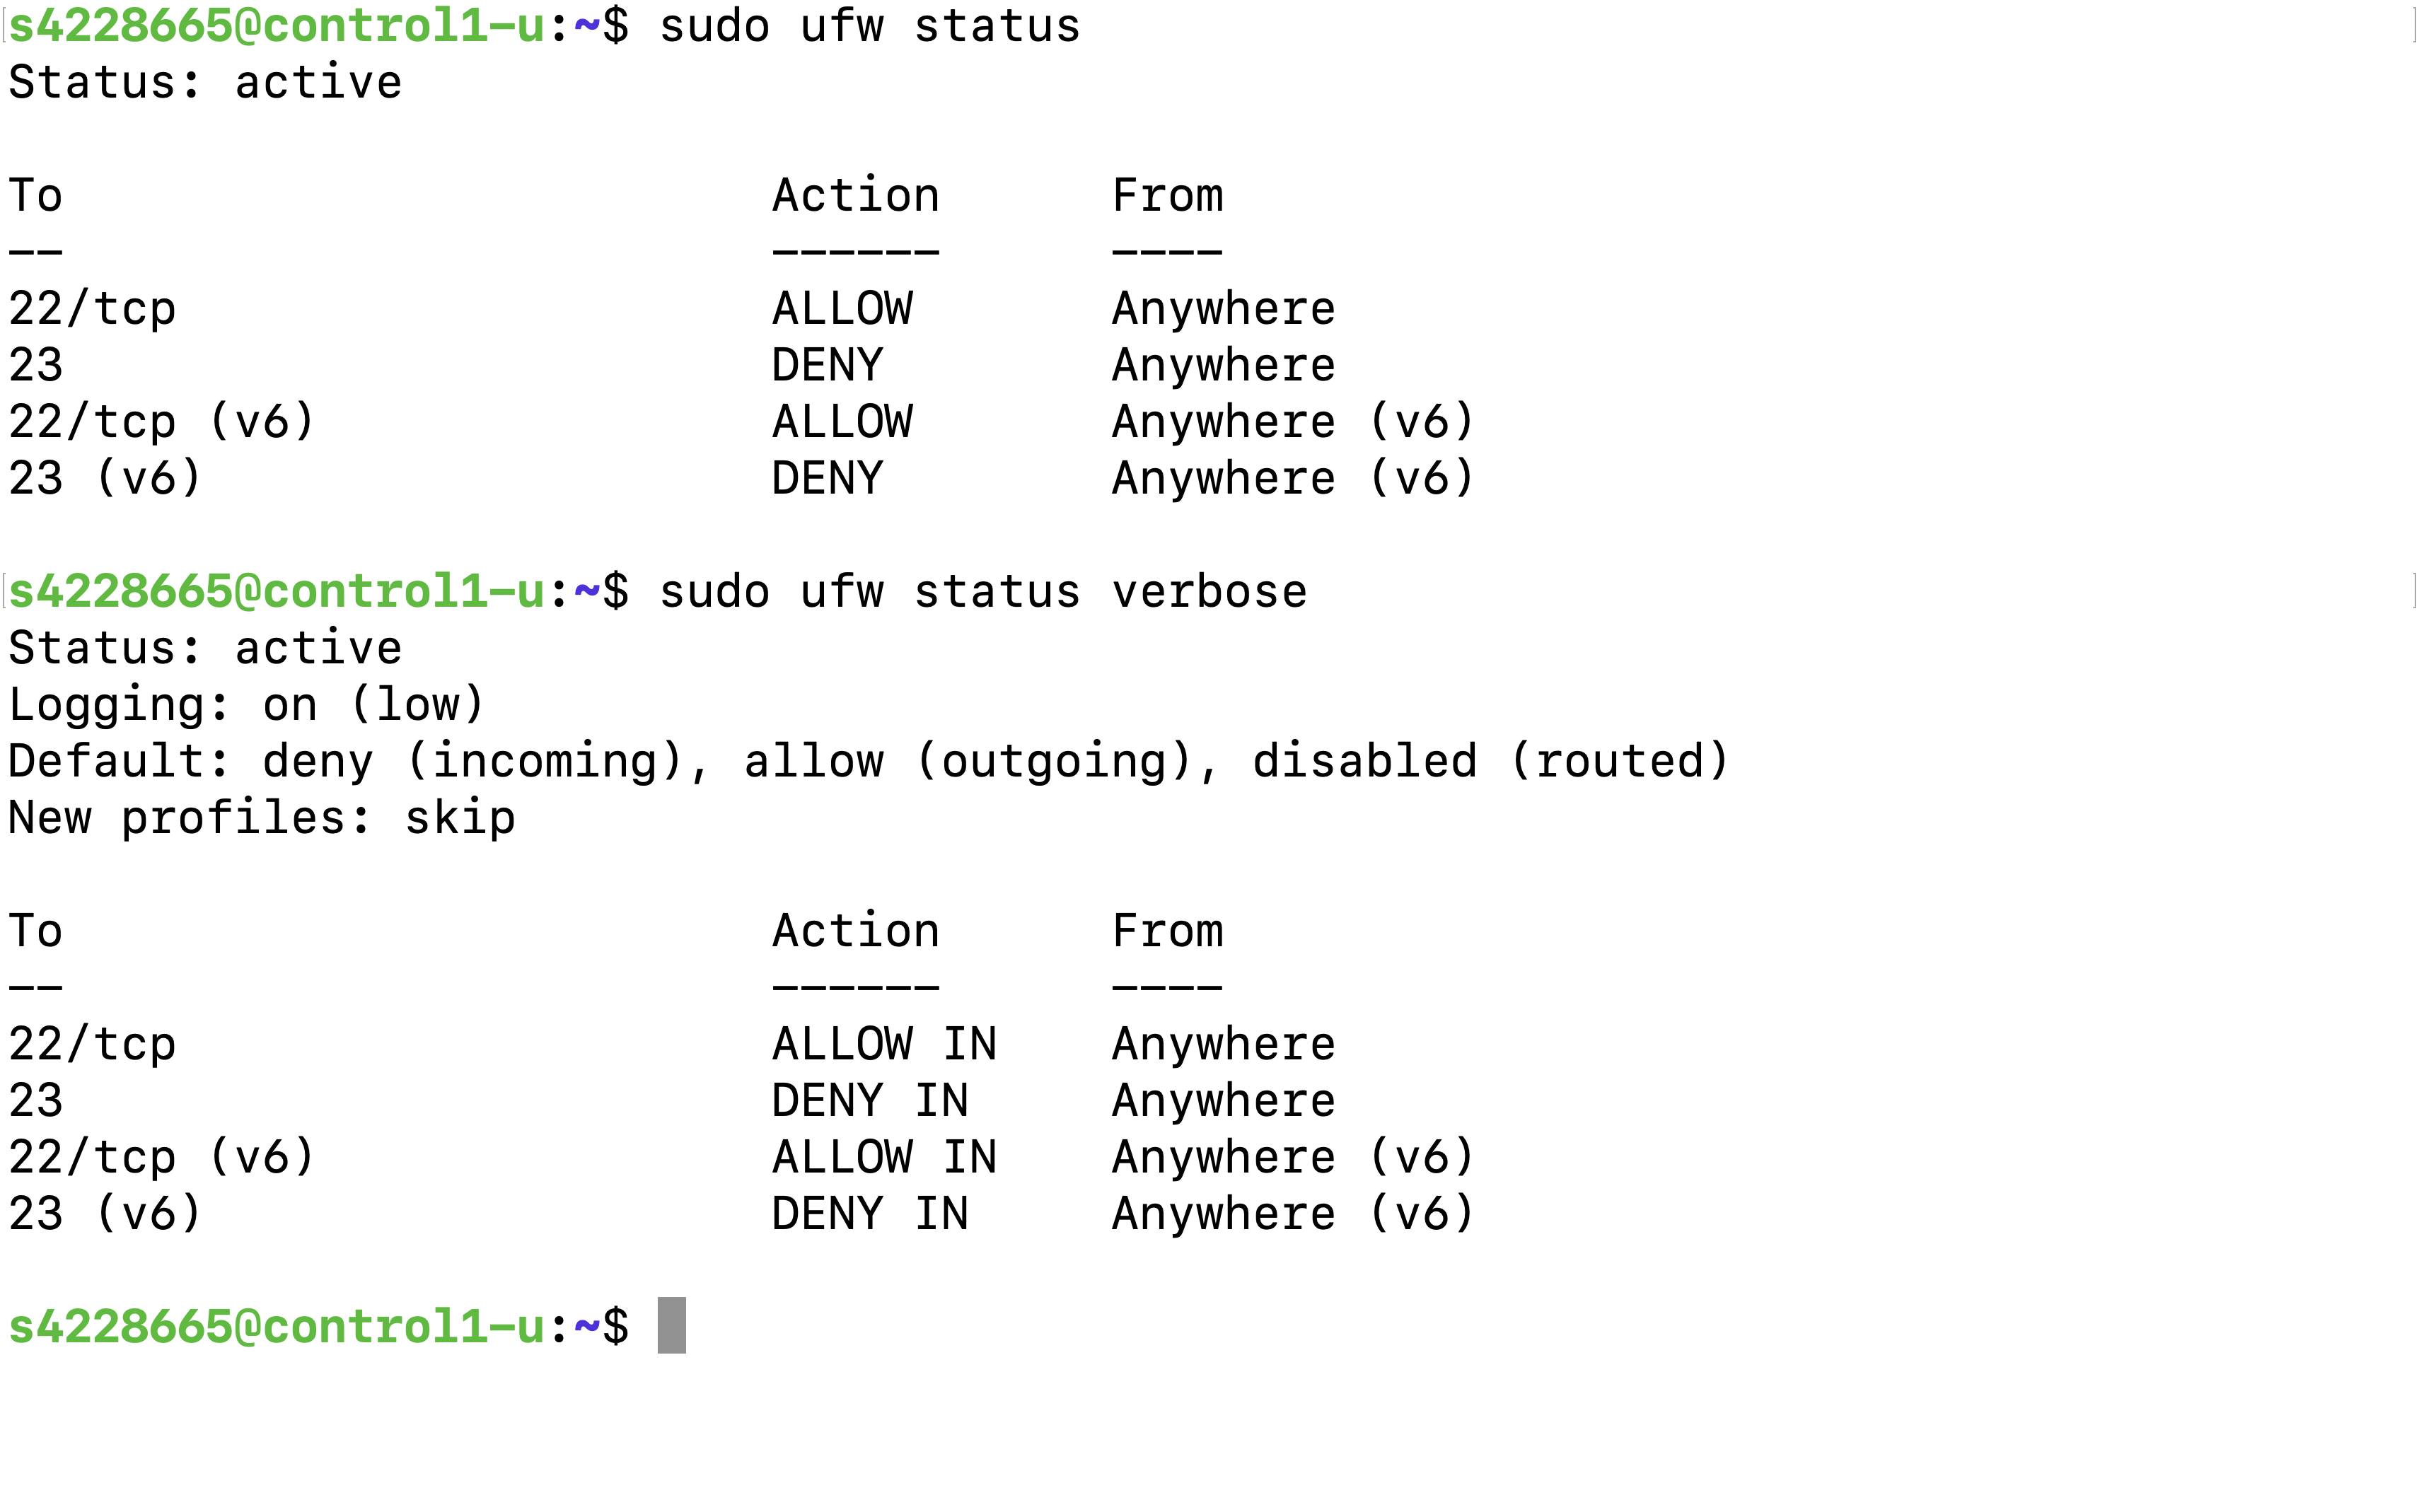
\includegraphics[width=0.8\linewidth]{Report_Images/os-ufw-screenshot.png}
    \caption{A screenshot from a Raspberry Pi running Ubuntu showcasing UFW policies to block port 23 (Telnet) and allow port 22 (SSH) connections. The verbose output shows the default rules of allowing all outgoing traffic but disabling default traffic going to the host.}
    \label{fig:UFW-example}
\end{figure}

To further secure a network, designers often segment it into different zones \parencite{paloalto2025privilege}, each with its own trust levels but still isolated from the others via firewall policies that allow only necessary traffic between networks. The coursework task also calls for this via an external Class-A network representing the untrusted internet connection, and two internal networks (Class-B and Class-C) simulating different frequency bands with different security requirements.

Following the "Never trust, always verify" approach \parencite{ravi2025beyond} to network security, firewalls should follow the principle of least privilege (PoLP) \parencite{paloalto2025segmentation}. PoLP works by limiting the amount of accessible data, resources, and applications to hosts/roles explicitly allowed to access them. Figure \ref{fig:UFW-example} does this by explicitly allowing only SSH connections instead of working and allowing SFTP (as an example) connections, which would be allowed if there were no firewall in place. This approach minimises the potential attack surface on the network and ensures that only necessary communications are allowed.

\subsection{Firewall OS Integration}
\label{subsec:os-integration}
To install an operating system on a typical (x86-based CPU) pc, you would create a boot medium. This can be done by installing the OS' image (.iso) file then running it through software that would take the .iso file and create a bootable usb-drive (or disk) that when inserted into the PC (and a user navigates to the boot options of the BIOS/UEFI) will boot to the install medium so a user can configure the OS install. This is how OPNsense would be installed on a supported x86 system. Unlike traditional x86-based hardware (in this case a firewall OS/distribution) that require installation to a storage medium, ARM-based systems like the Raspberry Pi require a different process. Instead of mounting the ISO image for installation, the Raspberry Pi requires a firmware image to be directly written (or "flashed") to the SD card, which serves as both the boot medium and primary (main) storage component

In discovering this, it was important to change plans to pick an implementation that would support the ARM-based CPU that the Raspberry Pi supports, as OPNsense only supports x86 CPUs. Another implementation of a network firewall is Ubuntu 24.04 with Iptables, an administration tool for IPv4 packet filtering and NAT \parencite{skilluped2020iptables}. This approach allows for a deeper understanding of Linux's netfilter kernel module and allows modern DevOps Infrastructure as Code practices (instead of using Opnsense's API) to be further explored in section \ref{sec:IaC}.

Ubuntu's netfilter framework, accessed through iptables, includes stateful packet inspection, network address translation (NAT), connection tracking, and logging \parencite{GeeksforGeeks2025iptables}. The system can be configured as a dedicated network gateway by enabling IP forwarding, configuring the three network interfaces (one USB-to-Ethernet adapter for the Class-A WAN interface, the built-in Ethernet for Class-B, and the onboard WiFi for Class-C as per figure \ref{fig:basic-fw-breakdown}), and implementing the required firewall changes through Iptables' rules. This approach aligns with professional practices where many enterprise firewalls are essentially hardened Linux systems running thier own implementation of Netfilter with custom software \parencite{IPv6Hawaii2024FirewallPerformance} like OpenWRT, the open source routing/firewall system \parencite{OpenWrt2024Official}.

\subsection{What is Iptables?}
Iptables is a command-line utility for configuring the packet filtering firewall in the Linux kernel's Netfilter framework \parencite{Linux2024IptablesManual}. The packet filtering is broken down into 3 different structures:
\begin{itemize}
    \item Tables \\
    This is the main mechanism behind iptables, as this is what is used to make decisions about whether a packet should be allowed to traverse the firewall, the main table of this implementation will be the filter table (there are also mangle, nat and raw tables that serve other features related to altering packet headers, routing based on NAT and even working with packets before hitting the kernel reads it) \parencite{BooleanWorld2024IptablesGuide}.
    \item Chains \\
    Tables are composed of different chains that do the packet filtering at various points of transmission though the firewall. Iptables has several chains but the ones used for this implementation are Input, Forward and Output, all associated with the filter table. Figure \ref{fig:iptables_breakdown} shows the chains and what tables they work with.
    \item Targets \\
    As the name suggests, targets determines where a packet ends up, if it's allowed though the firewall to a specific zone or if it's terminated and dropped from transmission depending on the rules/policies used.\parencite{DigitalOcean2024IptablesTutorial}
\end{itemize}

\begin{figure}[H]
    \centering
    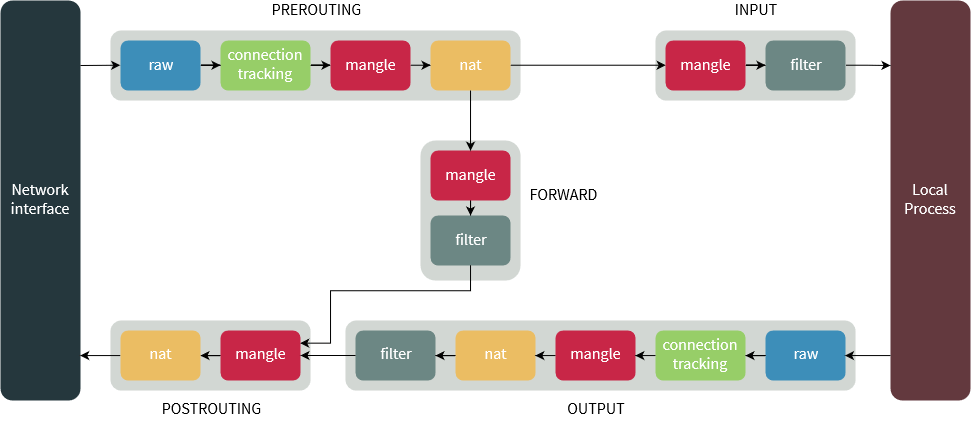
\includegraphics[width=0.8\textwidth]{Diagrams/os-iptables-chains.png}
    \caption{Iptables' chains and tables overview}
    \label{fig:iptables_breakdown}
    \parencite{BooleanWorld2024IptablesGuide}
\end{figure}

Using the same Raspberry Pi as seen in figure \ref{fig:UFW-example}, we can create another firewalling example of blocking icmp traffic using a simple iptables rule using the  example of An example of an iptables rule to block icmp traffic to a host using the \verb|input| table. First we can validate that icmp packets can hit the host, to test this we can ping the Raspberry Pi (figure \ref{example:iptables-ping-before}).


\begin{figure}[H]
  \centering
  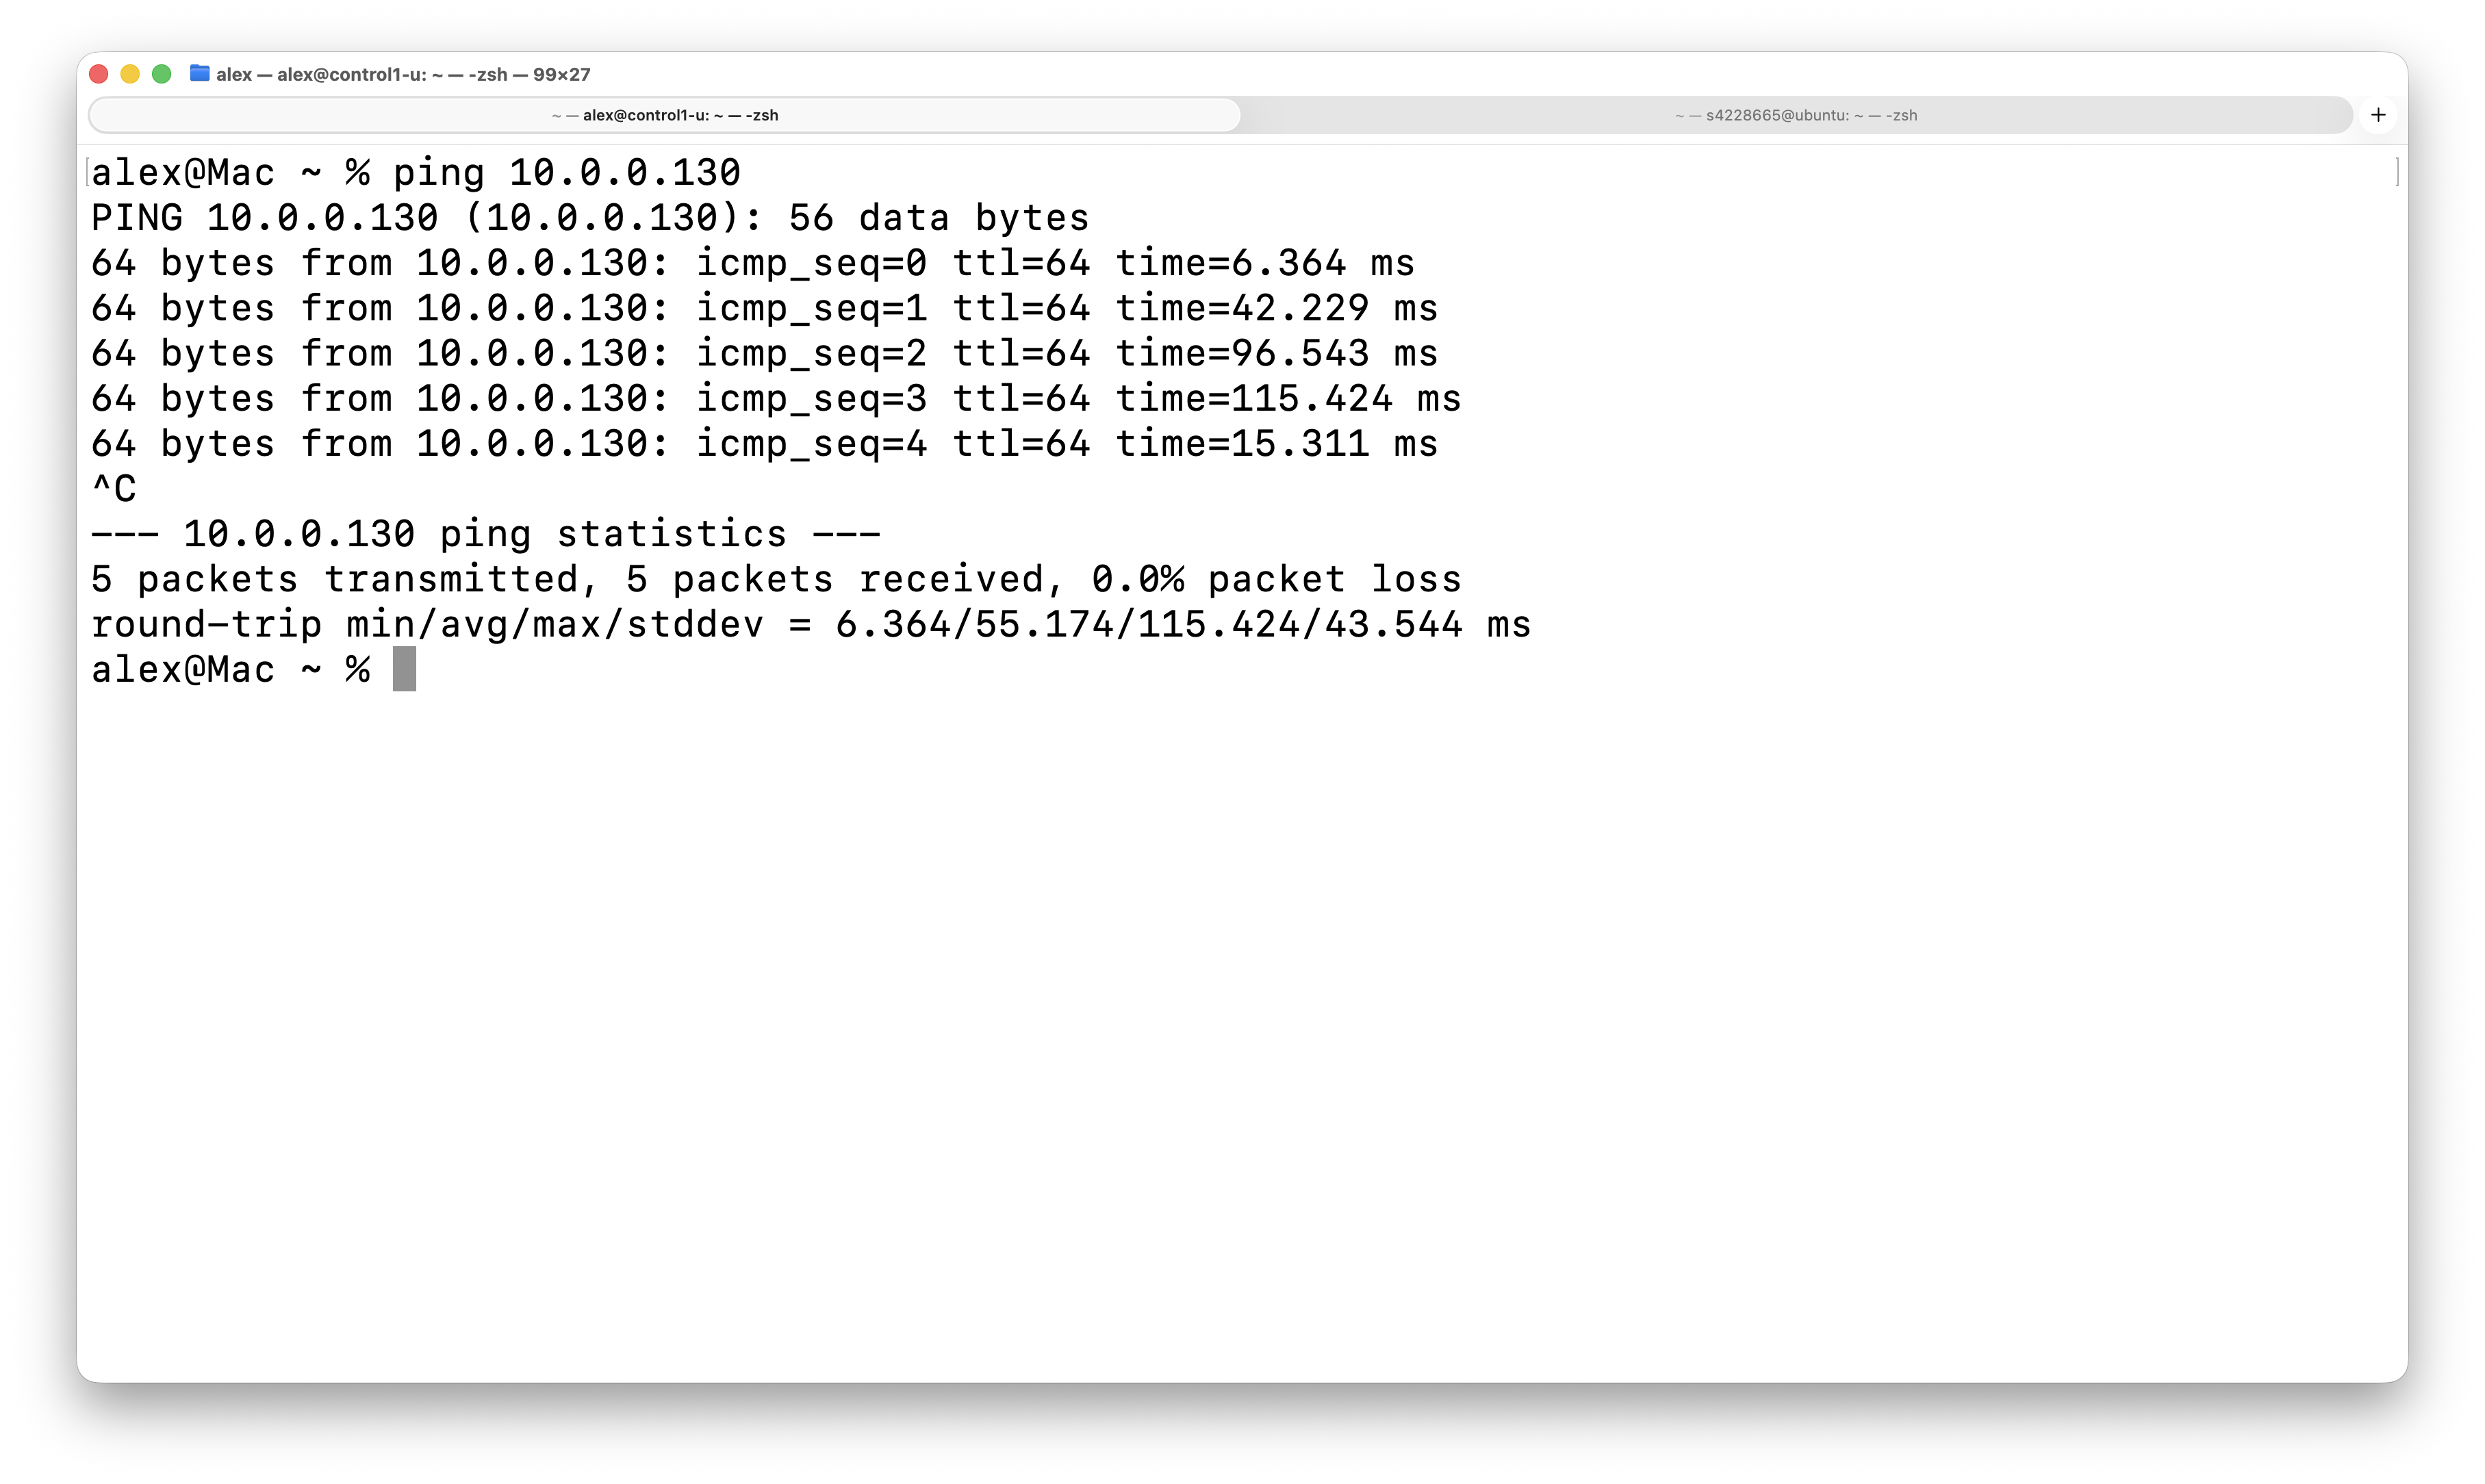
\includegraphics[width=0.8\linewidth]{Examples/iptables-ping-before.png}
  \captionof{figure}{A successful ping from my laptop to the Raspberry Pi}
  \label{example:iptables-ping-before}
\end{figure}

Since that has been validated, we can now put the rule in place to block the traffic, this is done using an iptables command but the coursework implementation will have this persisted using a file as seen later in section (TO DO REFERENCE DEPLOYMENT OF IPTABLES CONFIG FILE). The command for this is \verb|sudo iptables -A INPUT -p icmp -j DROP| which is to access the iptables cli, \verb|-A| to append to the \verb|INPUT| chain, \verb|-p| to specify we're dealing with \verb|icmp| traffic (protocol) and \verb|-j| to 'Jump' to a specified target, and we're going to \verb|DROP| it \parencite{Ubuntu2024IptablesHowTo}.

To validate the host is online and not just off (as ping tests are used to determine if a host is online) we can add a second rule to log the dropped packets, at base iptables does not log unless specified, so we can add a rule to log what happens to the incoming icmp traffic (CITATION). This command is \verb|sudo iptables -A INPUT -p icmp -j LOG --log-prefix "Blocked_icmp"|, the same levels of access as the previous rule to append to the \verb|input| chain but the \verb|-j| is jumping to the \verb|LOG| target where we can append the log using \verb|--log-prefix| with \verb|Blocked_icmp| to grep though system logs later.

\begin{figure}[H]
  \centering
  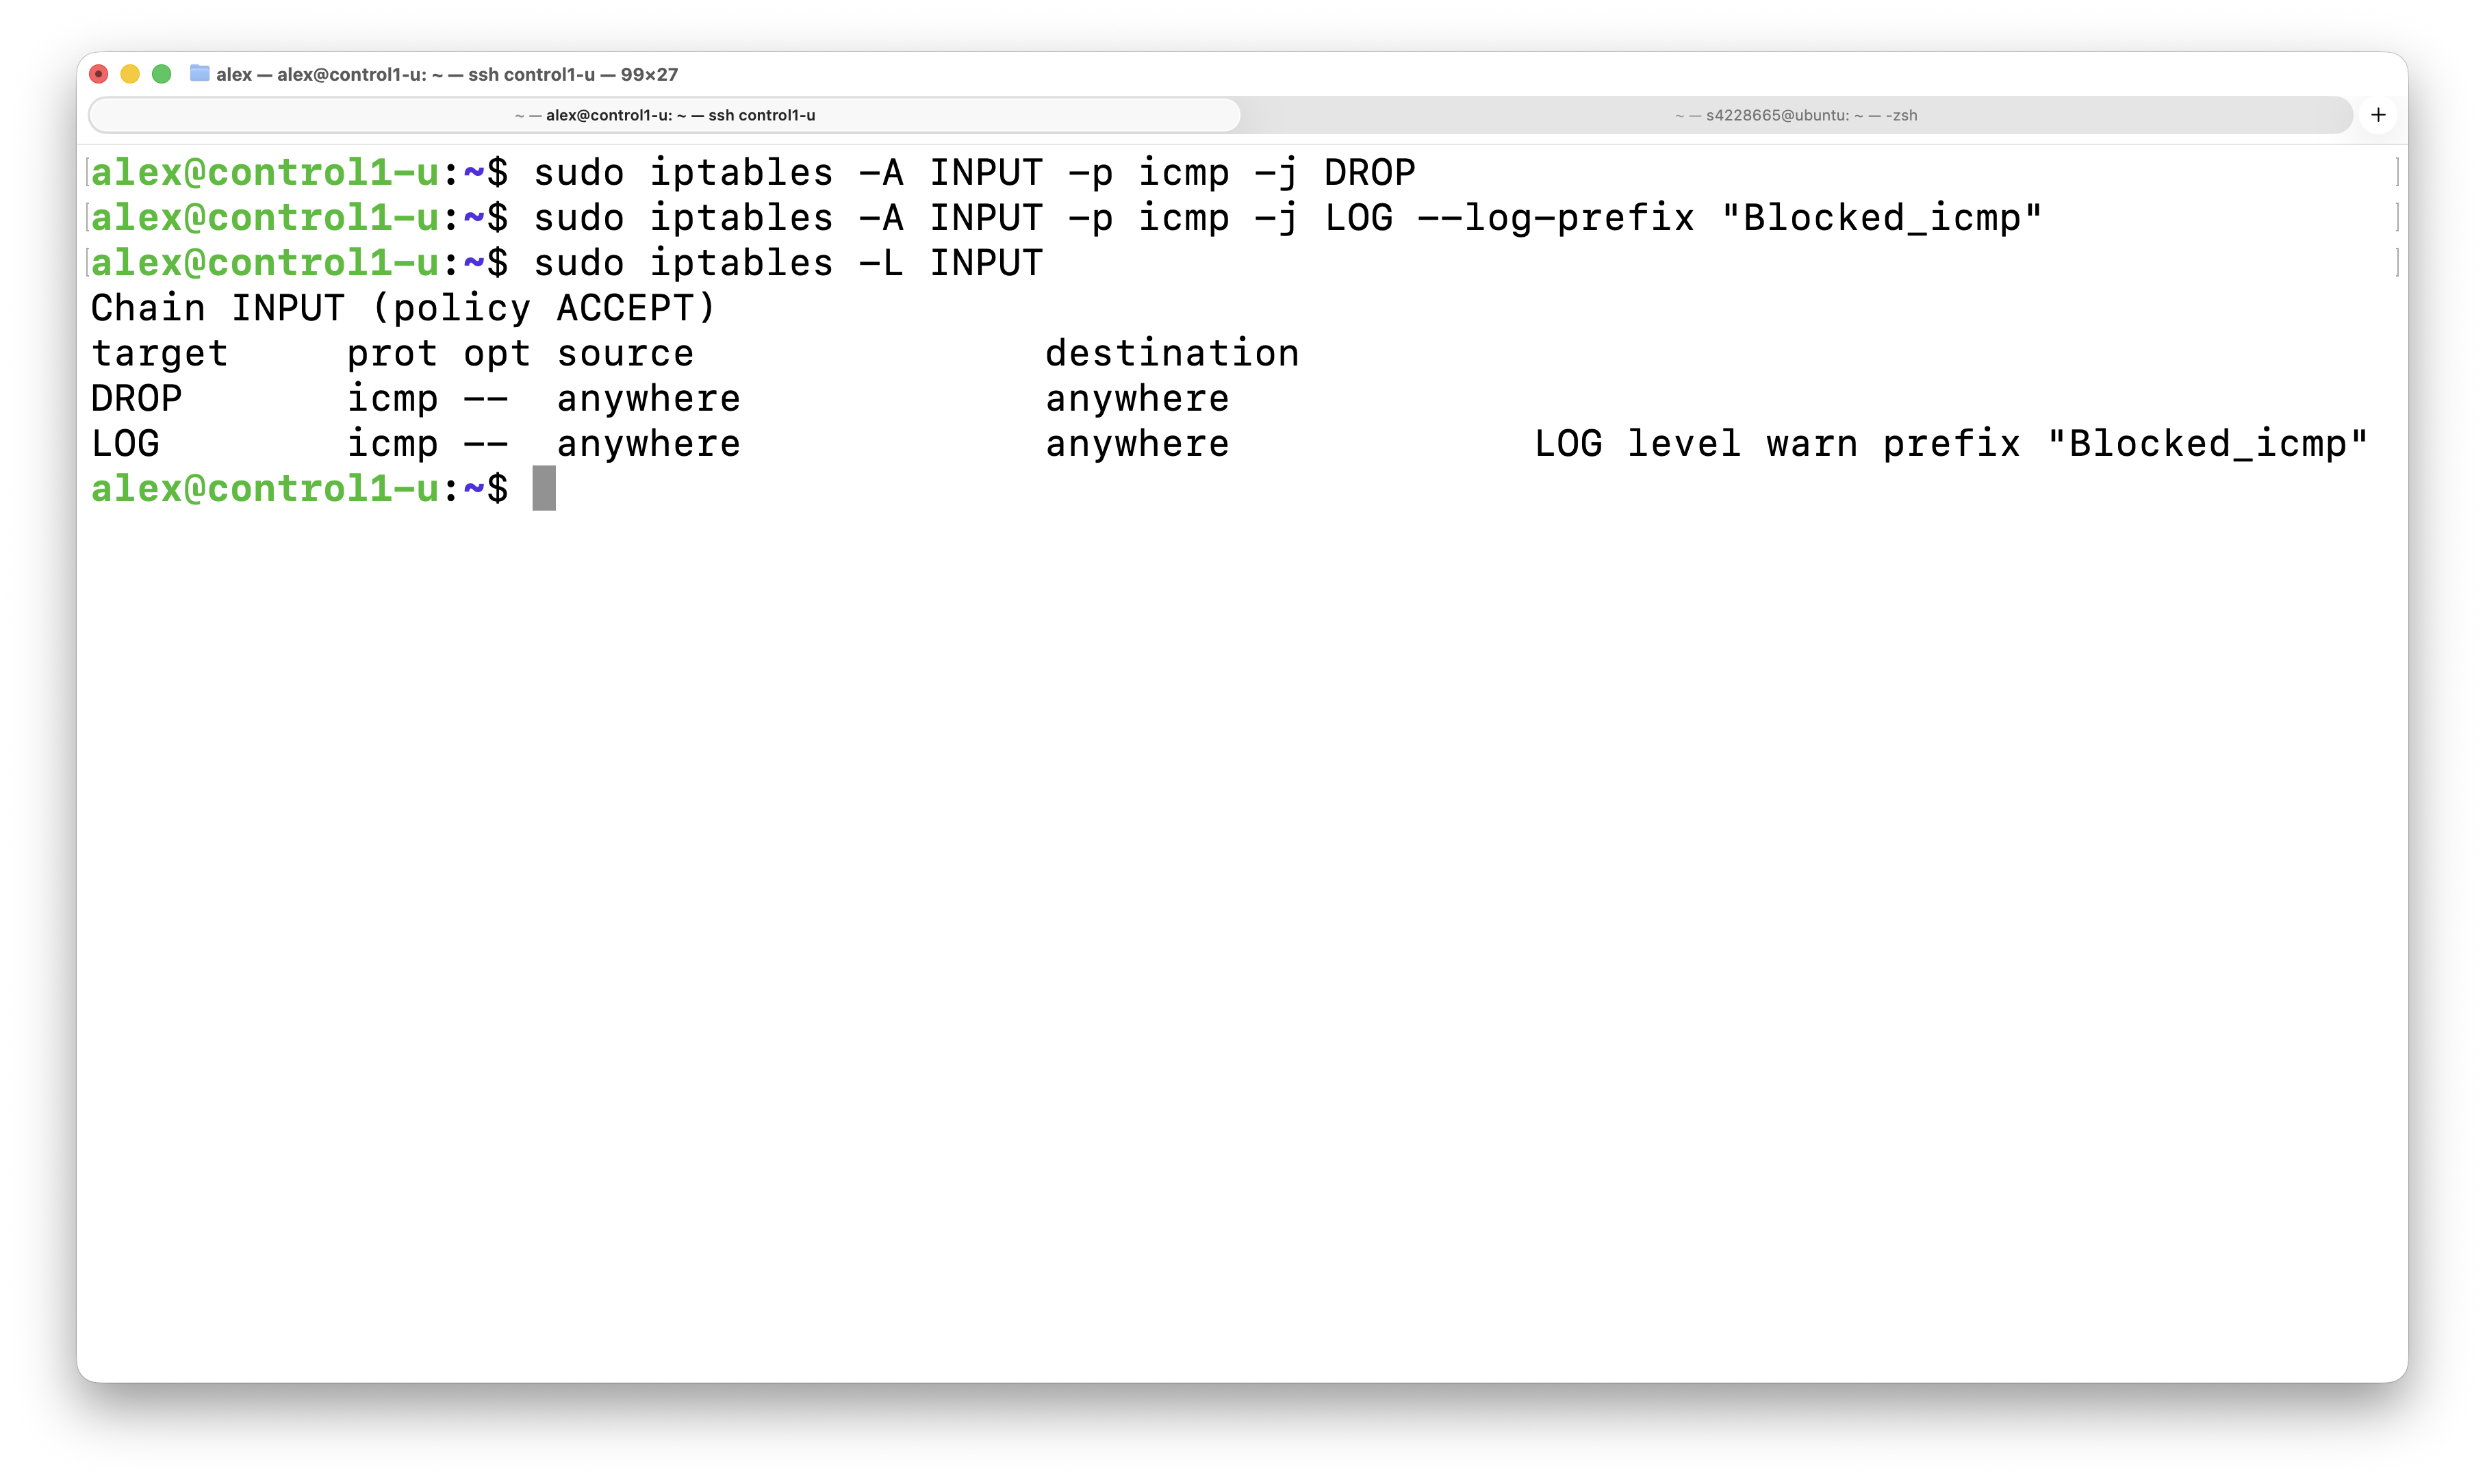
\includegraphics[width=0.8\linewidth]{Examples/iptables-ping-rules.png}
  \caption{Iptables rule in place to block all incoming icmp traffic  another to log the packets}
  \label{example:iptables-rules}
\end{figure}

We can now check this by sending icmp traffic to the now basic firewall and check the logs (stored in \verb|/var/log/syslog| by default) to see how the firewall dealt with the packets.

\begin{figure}[H]
    \centering
    \begin{subfigure}[b]{0.49\textwidth}
        \centering
        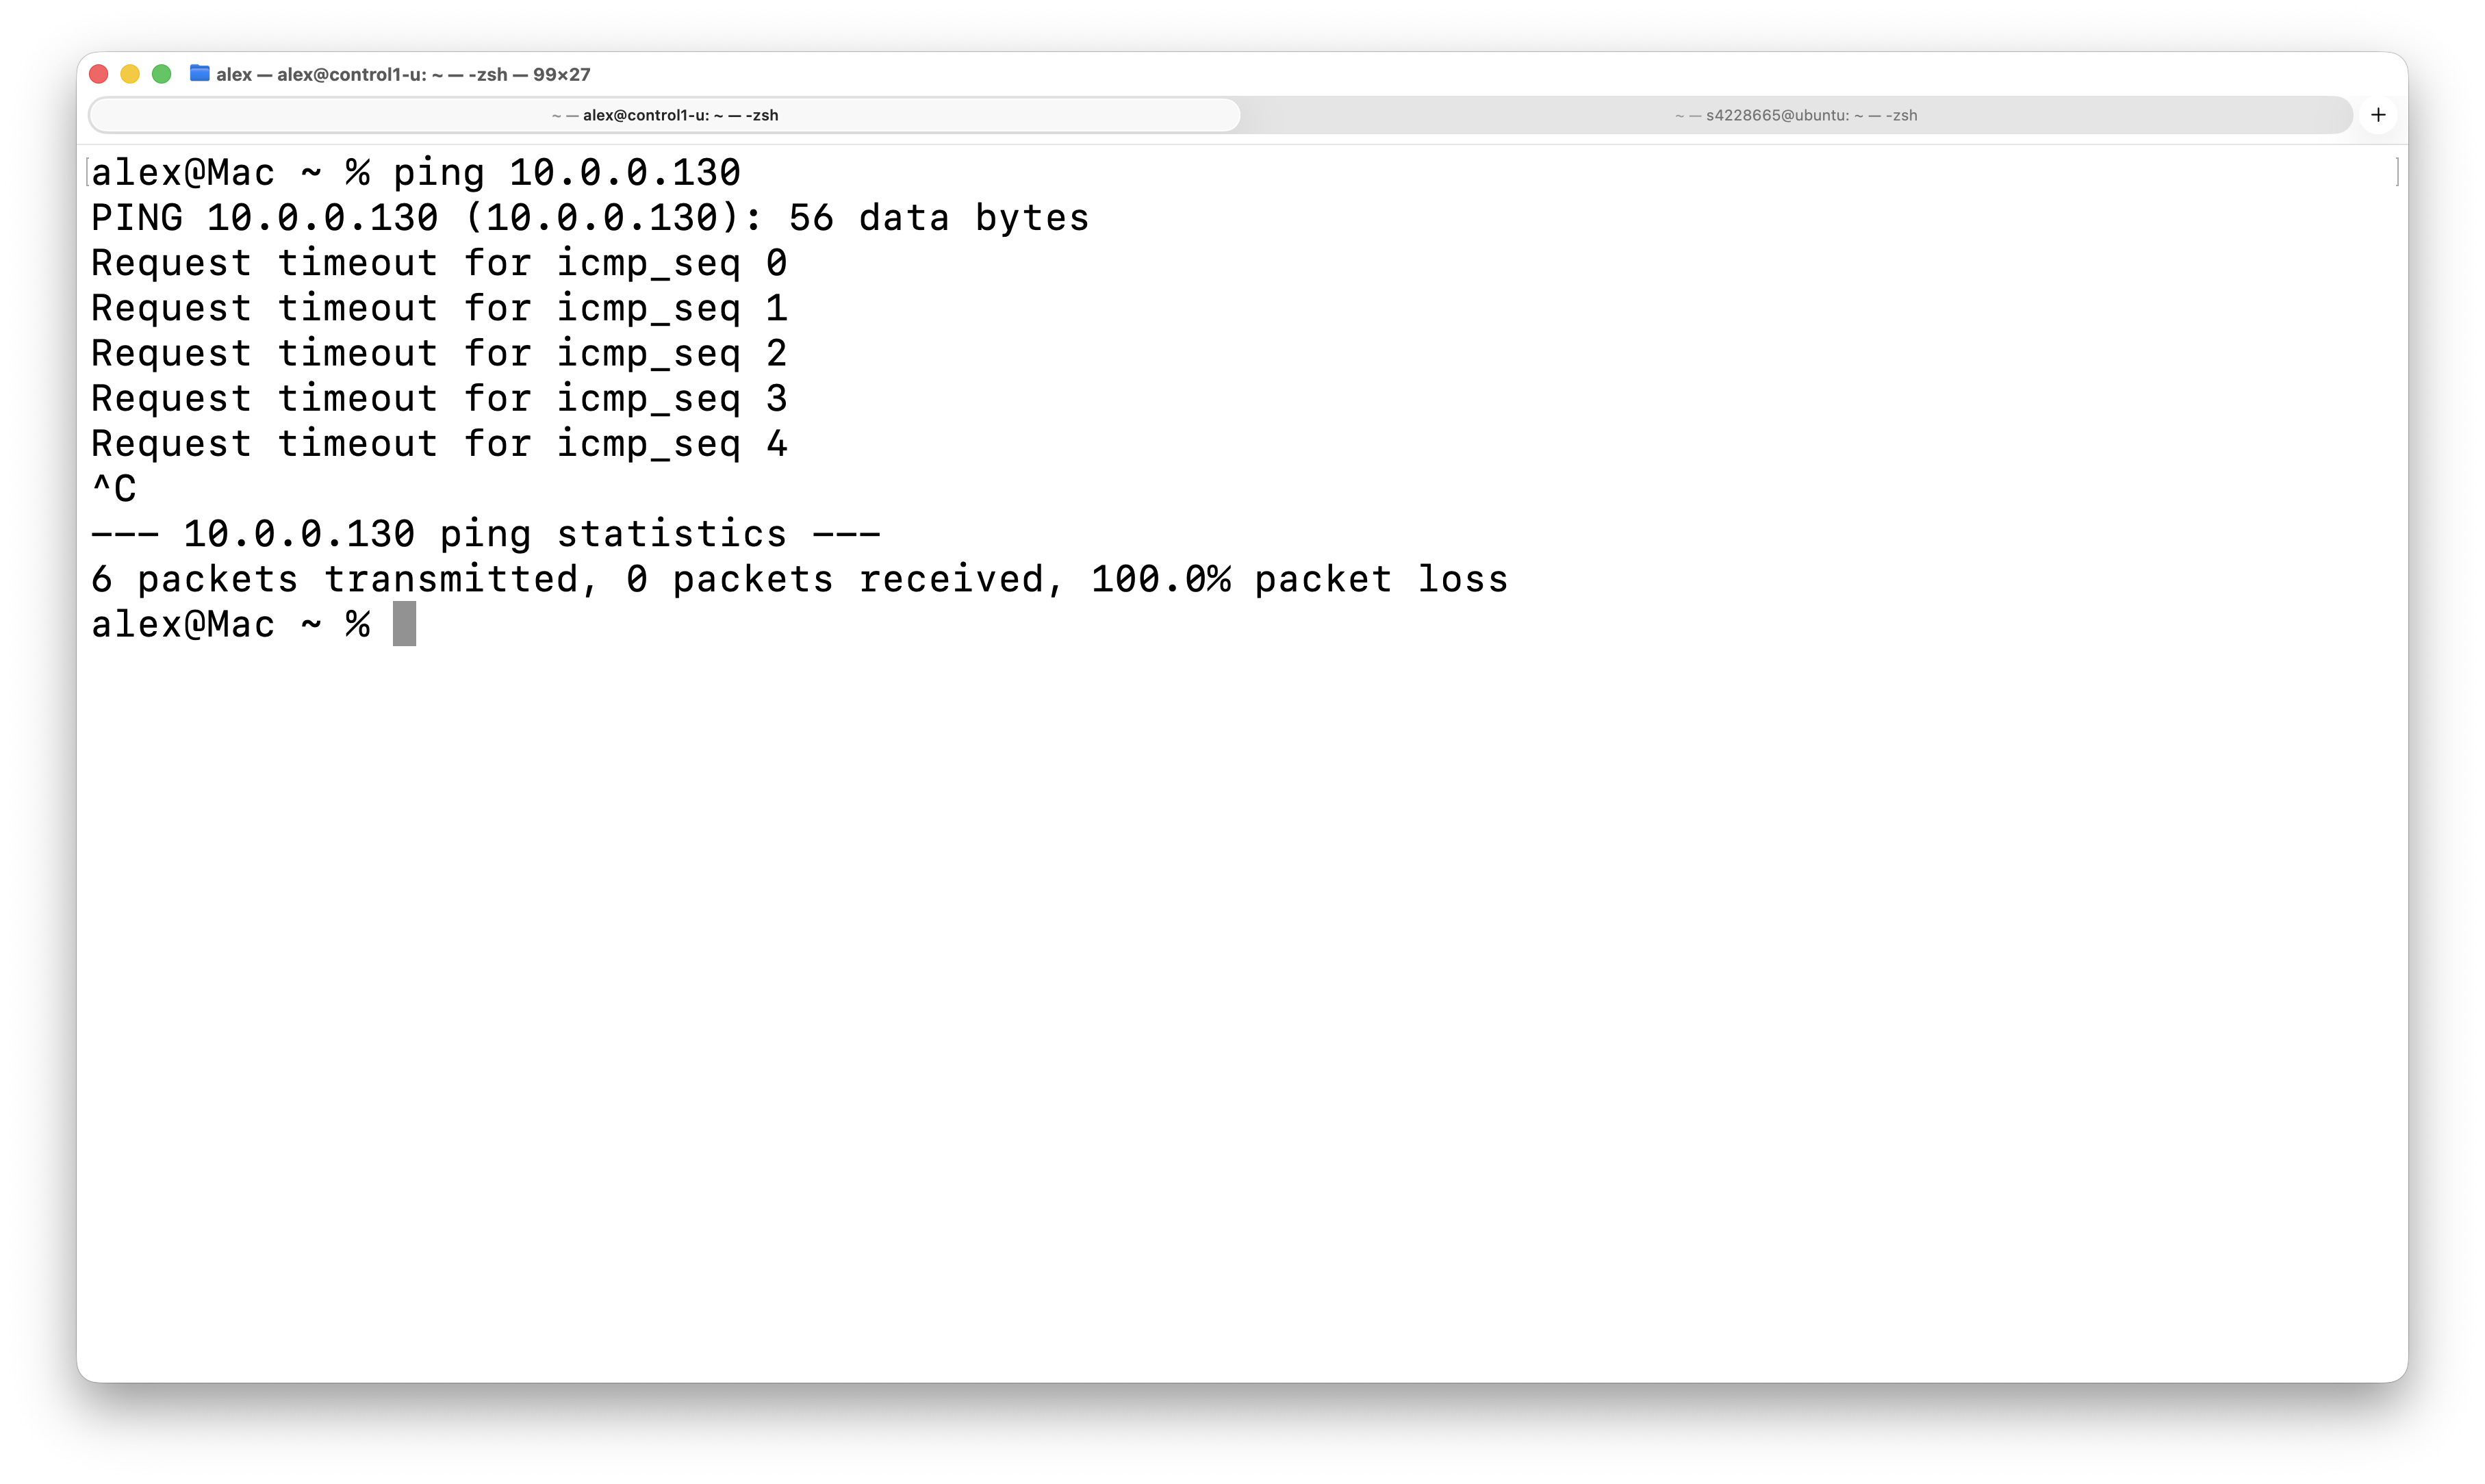
\includegraphics[width=\textwidth]{Examples/iptables-ping-blocked.png}
        \caption{A blocked successful ping from my laptop to the Raspberry Pi}
        \label{example:iptables-ping-blocked}
    \end{subfigure}
    \hfill
    \begin{subfigure}[b]{0.49\textwidth}
        \centering
        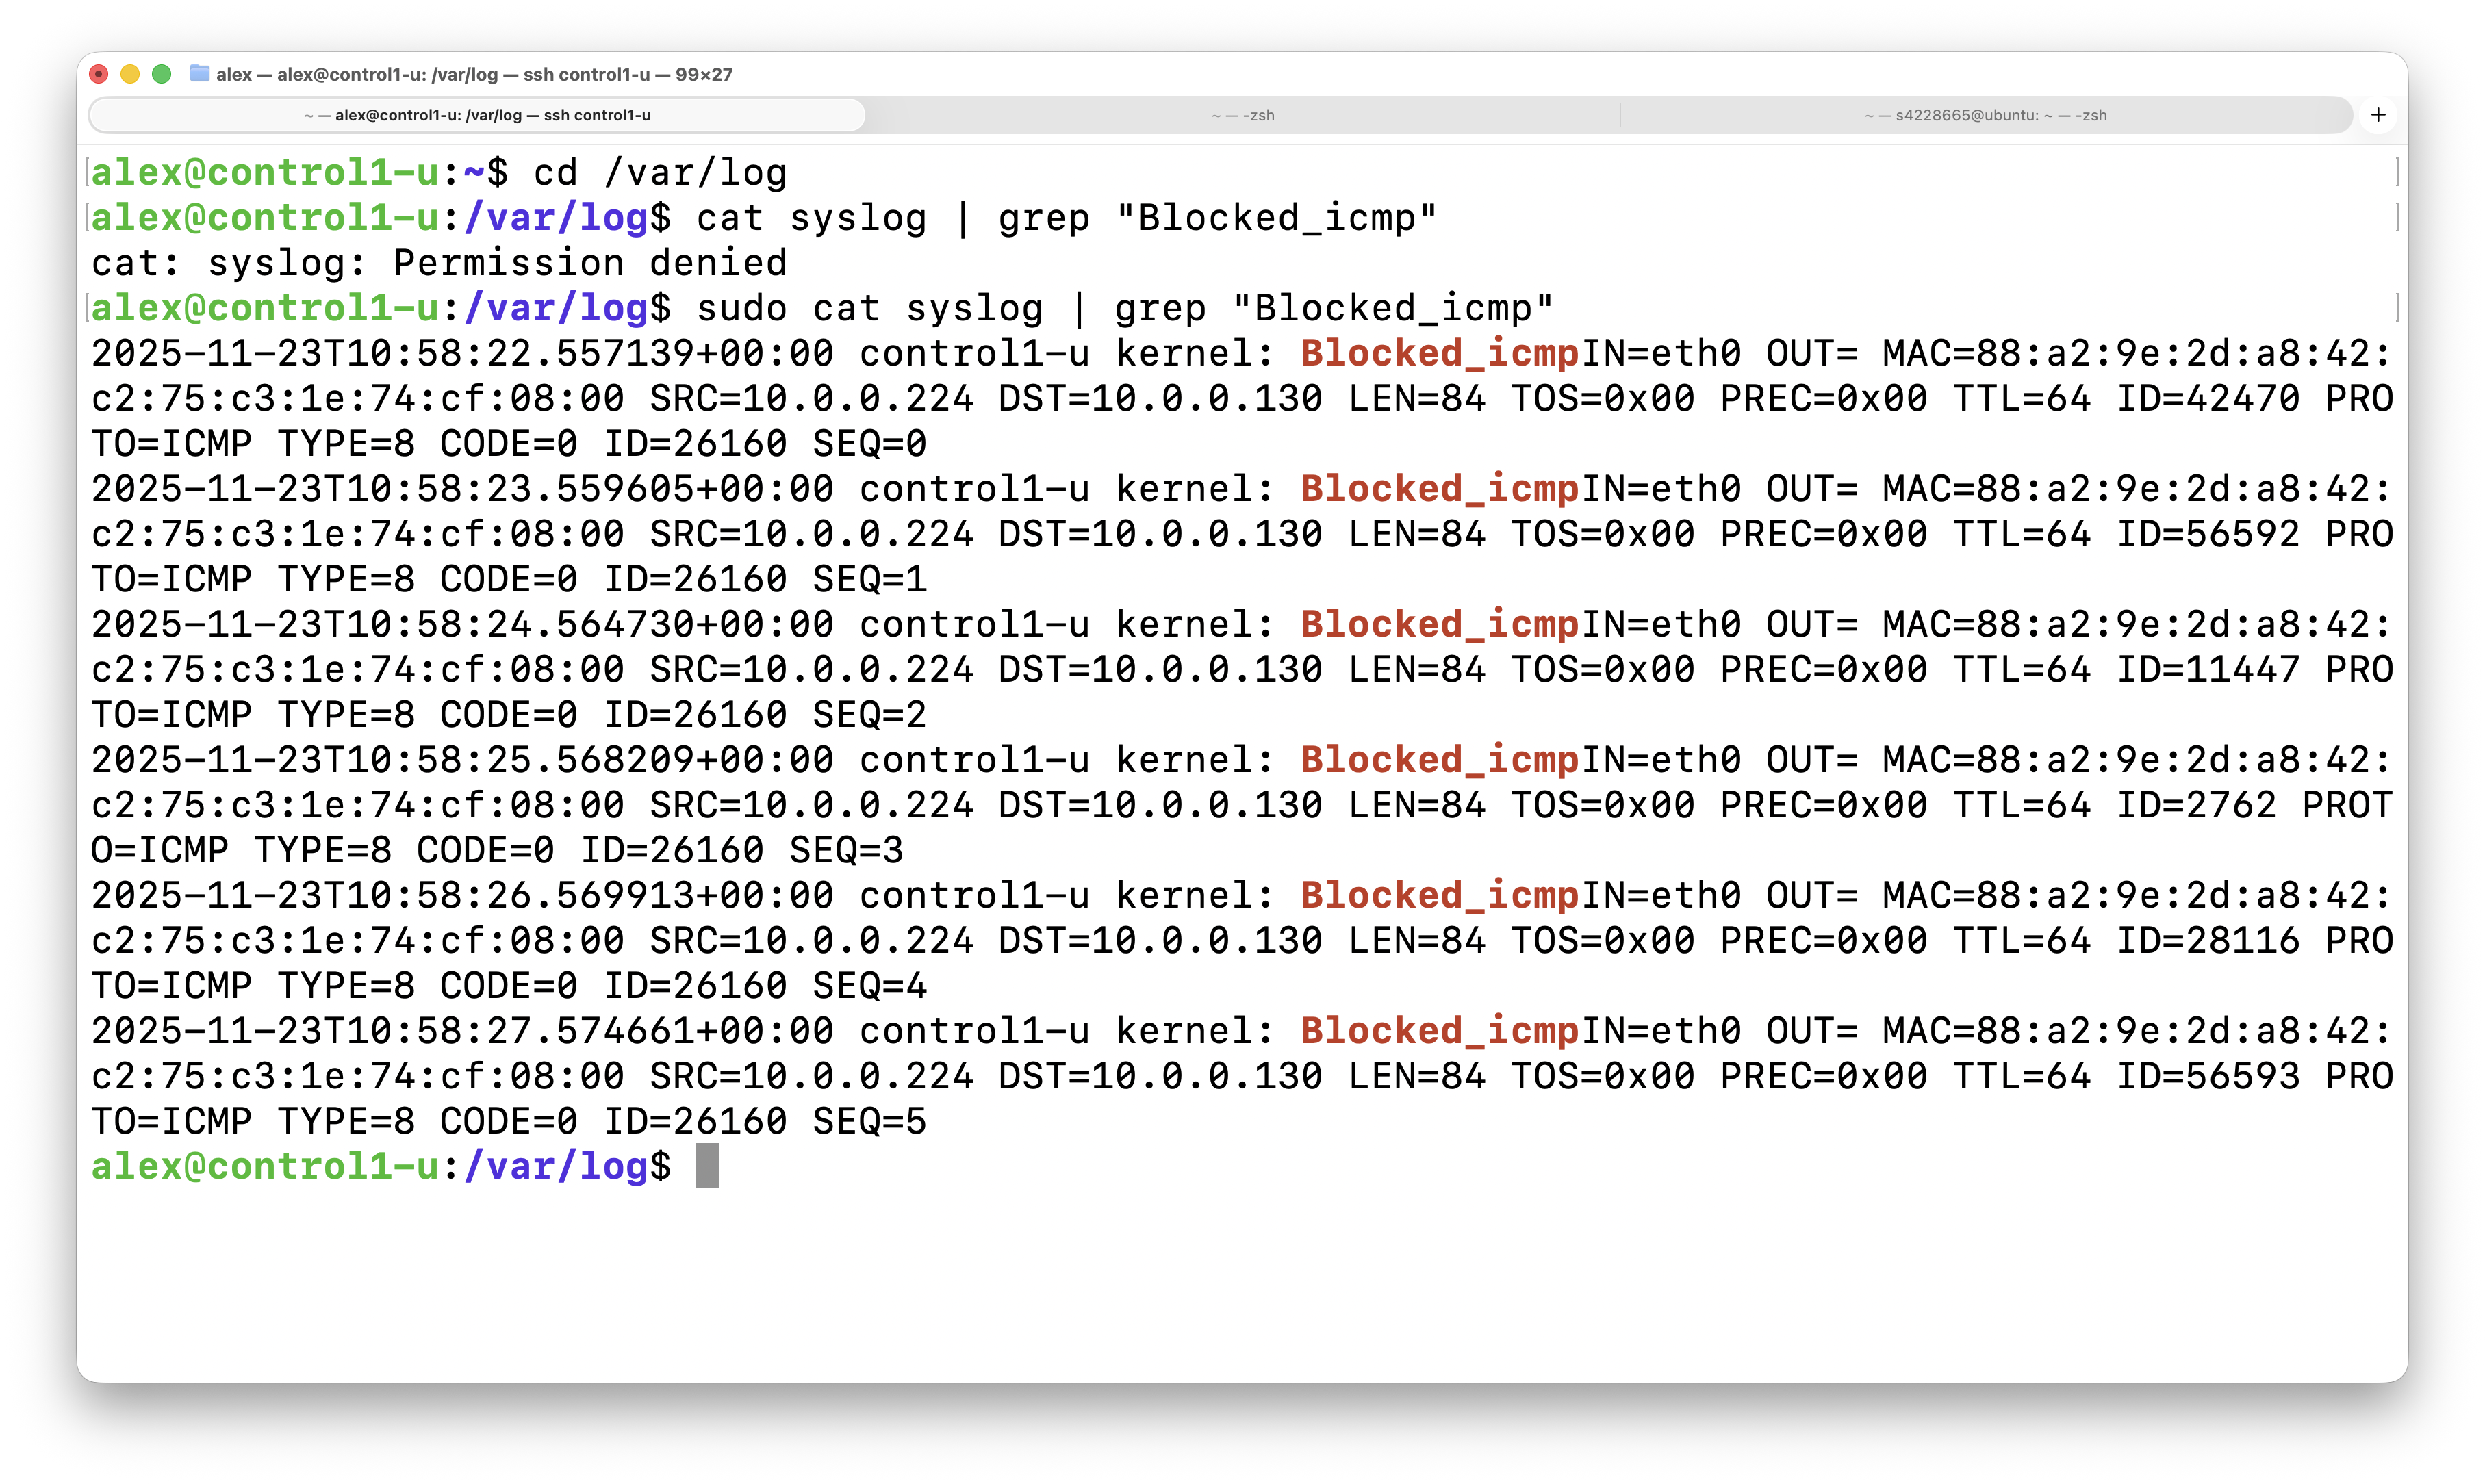
\includegraphics[width=\textwidth]{Examples/iptables-ping-logs.png}
        \caption{Logs from the iptables rule showing the dropped packets}
        \label{example:iptables-logs}
    \end{subfigure}
    \caption{Side-by-side view of the blocked ICMP traffic and the corresponding iptables logs}
    \label{fig:side-by-side-iptables-1}
\end{figure}

We can see the blocked pings in \ref{example:iptables-ping-blocked} and the corresponding logs in \ref{example:iptables-logs}. While iptables can't show the actions taken for each packet, the start of both rules (\verb|iptables -A INPUT -p icmp|) links them as they're both dealing with \verb|icmp| packets. From this we can also see the following about the packet:
\begin{itemize}
    \item The source's (My laptop) MAC address \verb|MAC=88:a2:9e:2d:a8:42:c2:75:c3:1e:74:cf:08:00|
    \item The source's IP address \verb|SRC=10.0.0.224|
    \item The destination's (My Pi) IP address \verb|DST=10.0.0.130|
    \item The protocol \verb|PROTO=ICMP|
\end{itemize}

As I use icmp packets to confirm if the Pi is online, I will remove the rules and validate packets are able to flow as intended in figures \ref{example:iptables-ping-after} and \ref{example:iptables-after}.

\begin{figure}[H]
    \centering
    \begin{subfigure}[b]{0.49\textwidth}
        \centering
        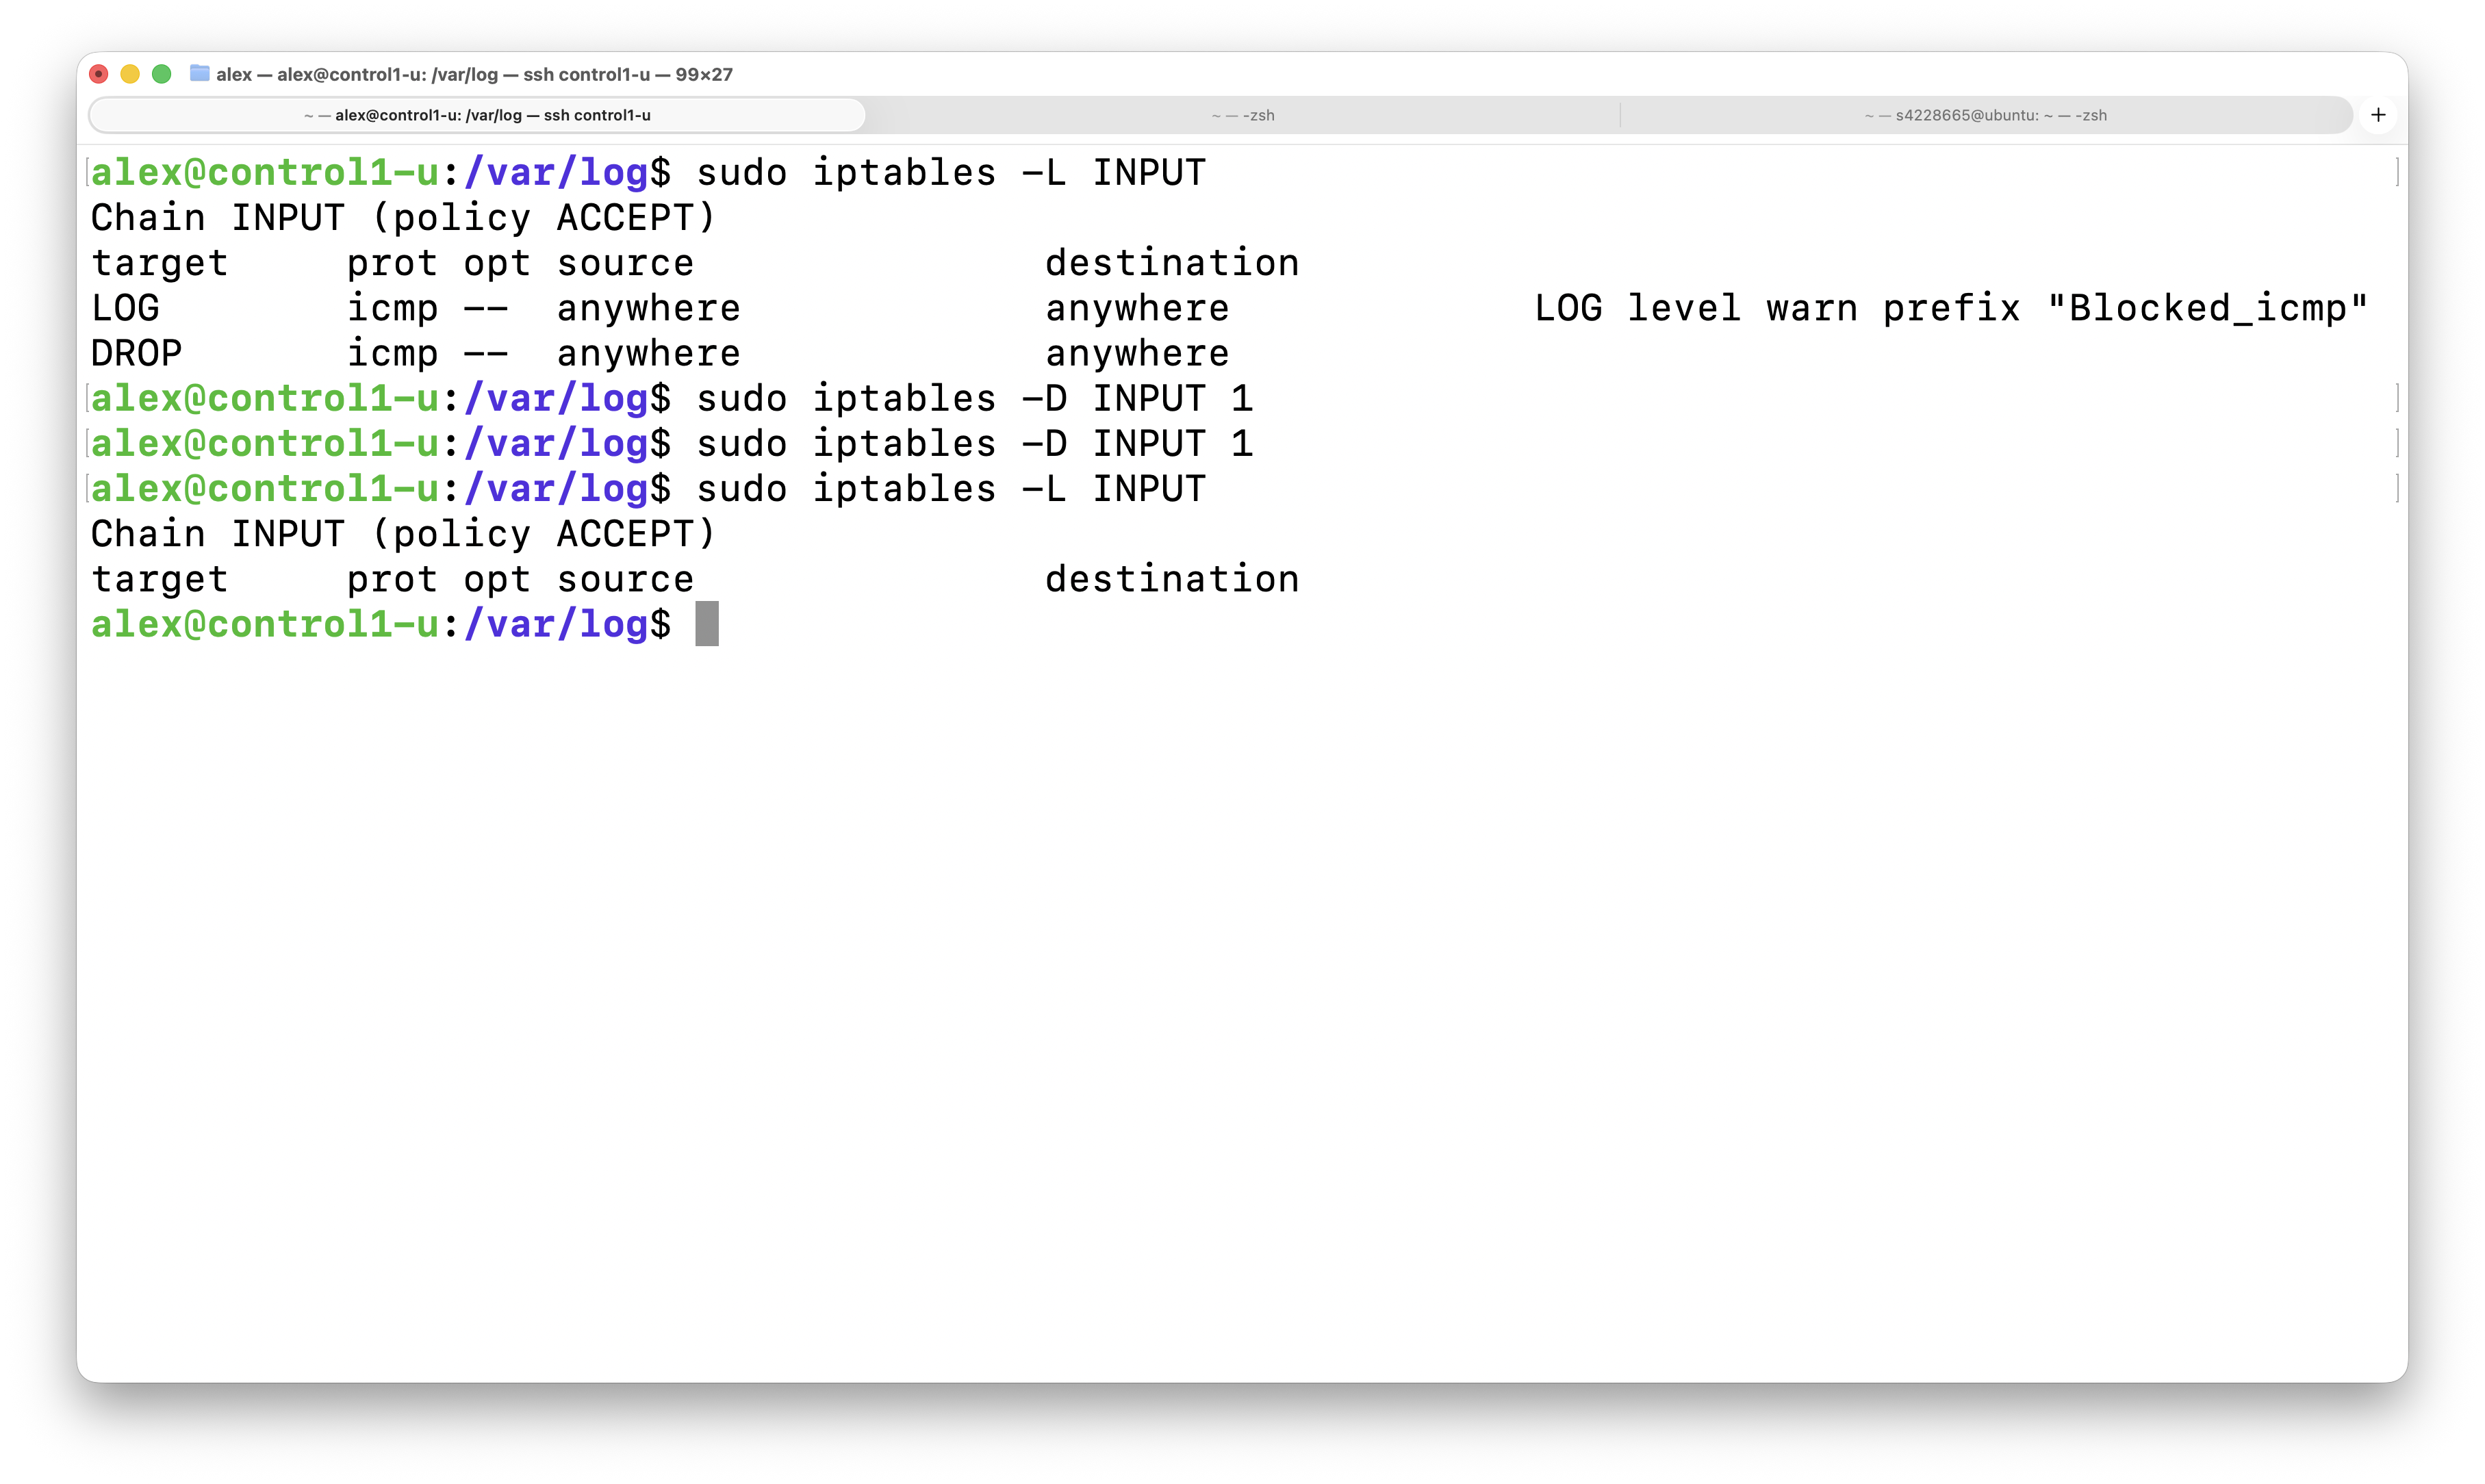
\includegraphics[width=\textwidth]{Examples/iptables-ping-cleanup.png}
        \caption{Both icmp iptables rules deleted showing zero 'input' rules}
        \label{example:iptables-ping-after}
    \end{subfigure}
    \hfill
    \begin{subfigure}[b]{0.49\textwidth}
        \centering
        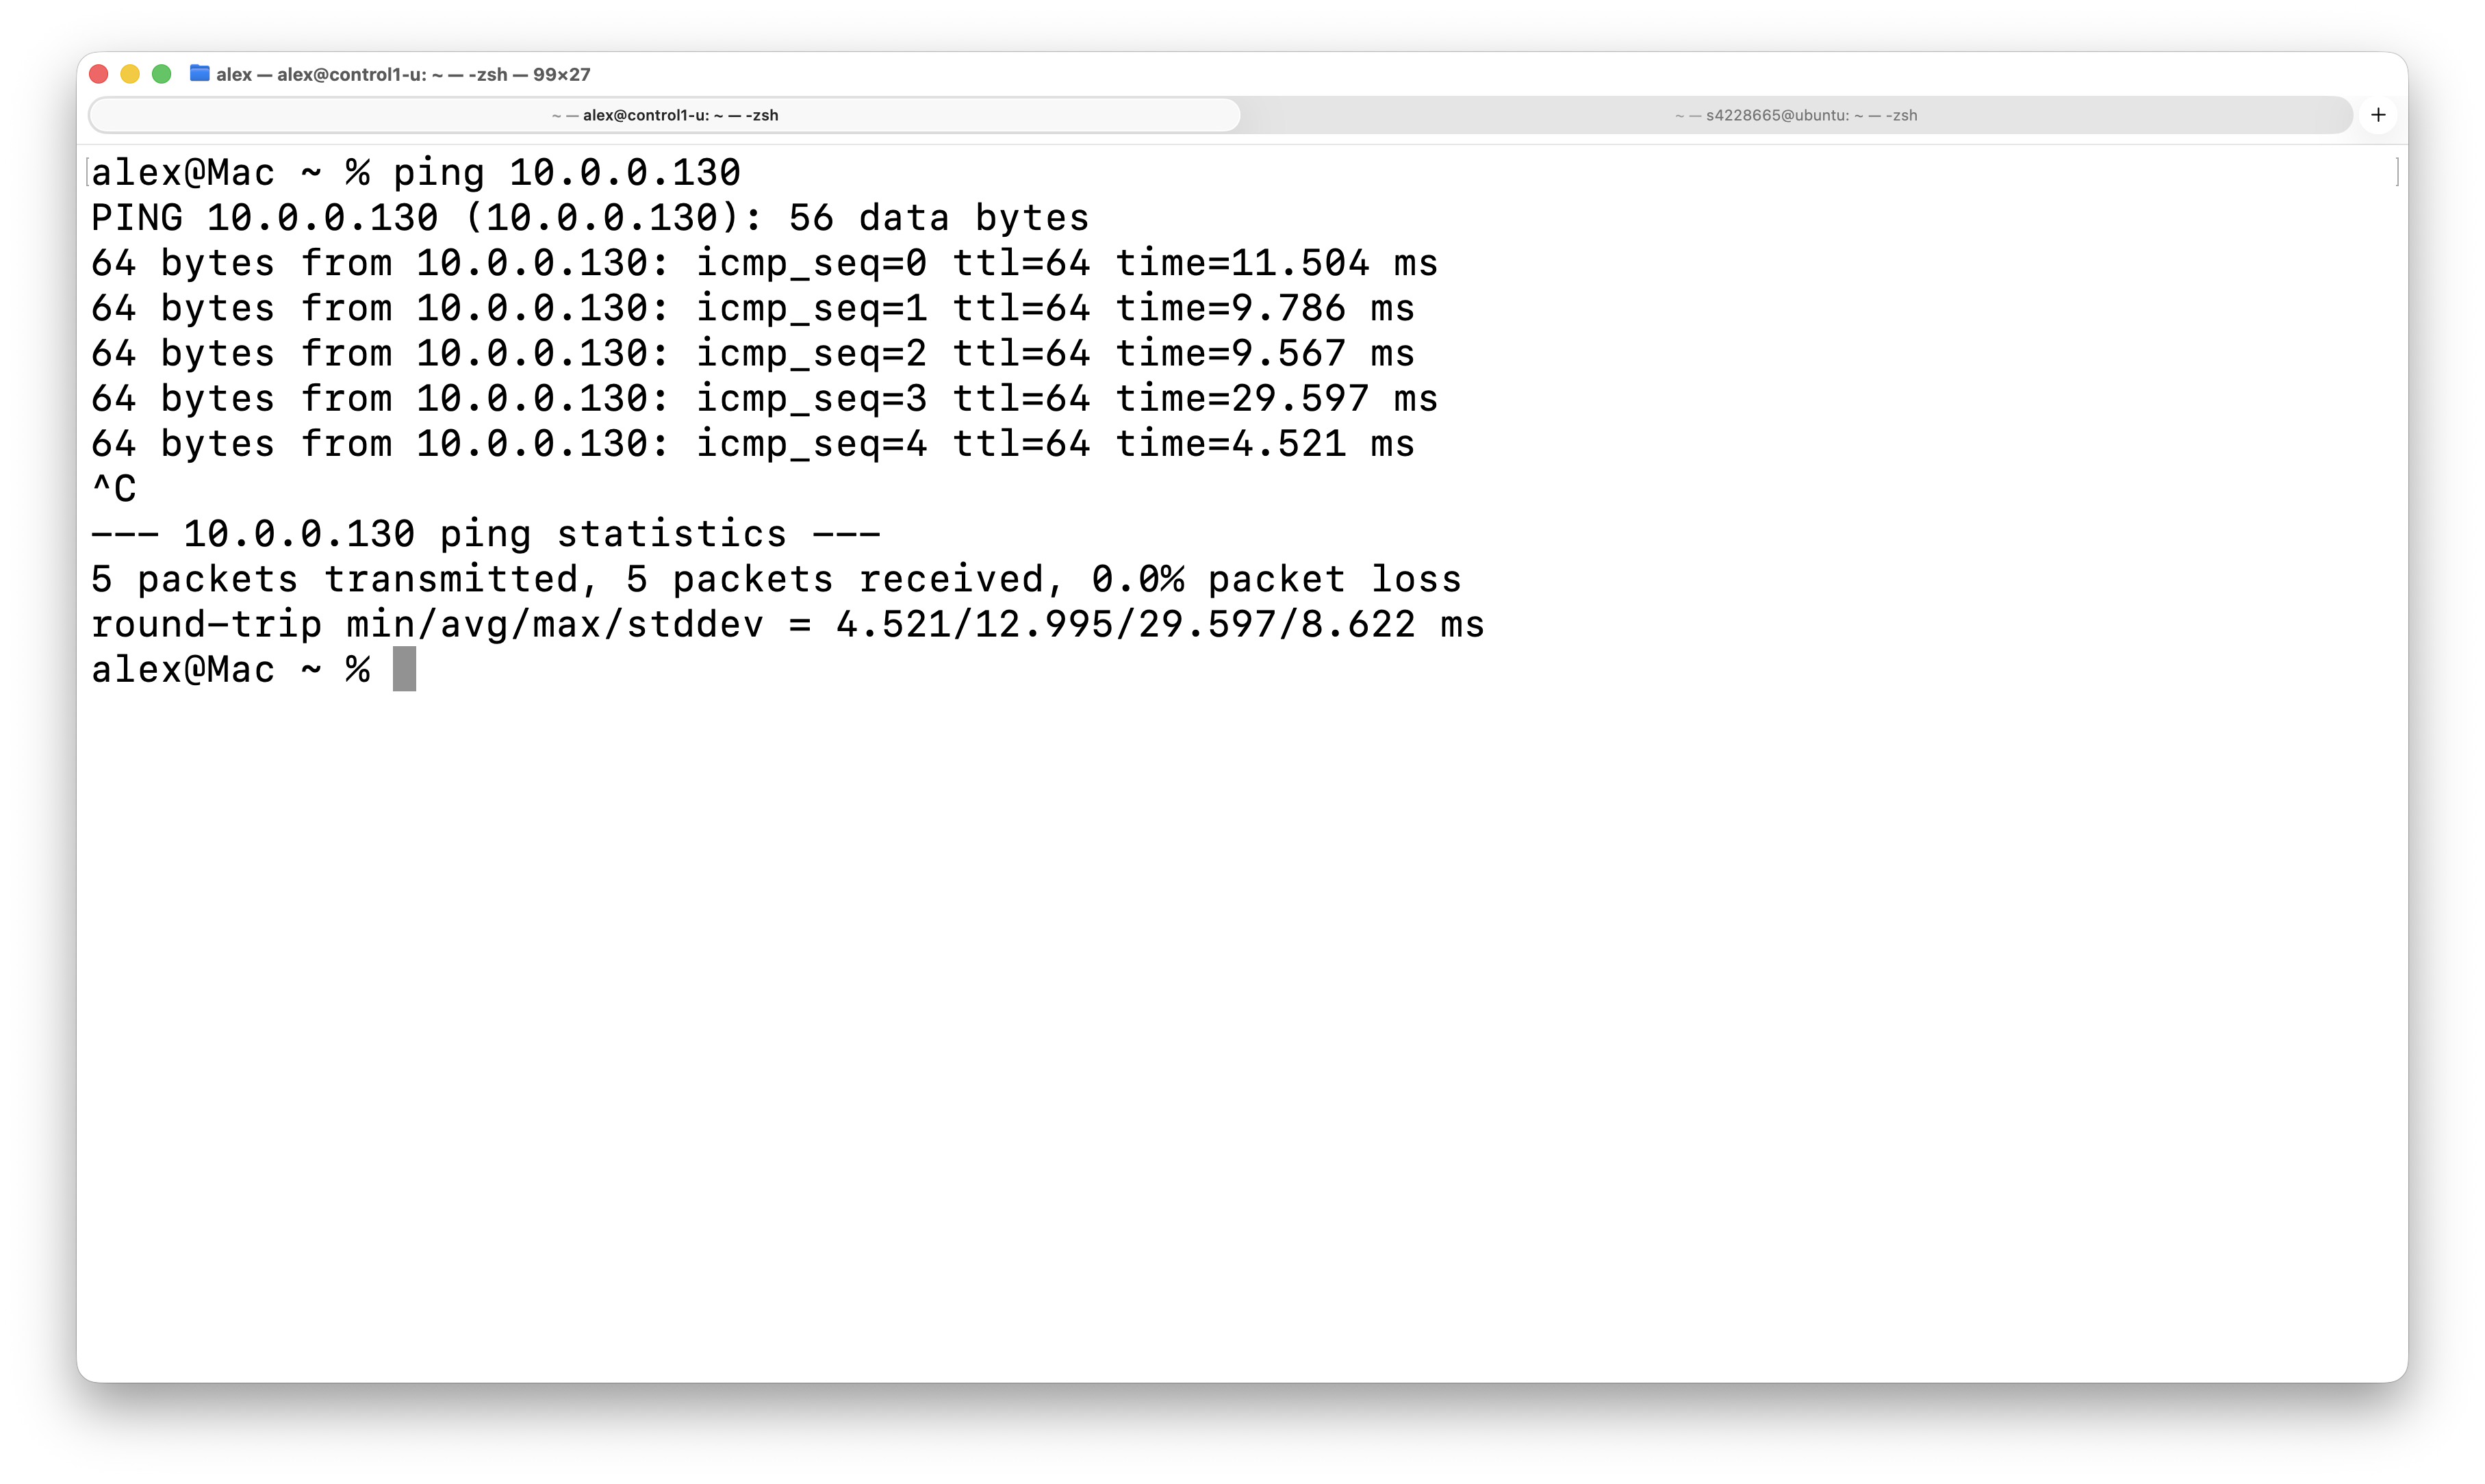
\includegraphics[width=\textwidth]{Examples/iptables-ping-after.png}
        \caption{Successful pings hitting the Pi after the icmp blocking rules were removed}
        \label{example:iptables-after}
    \end{subfigure}
    \caption{Side-by-side view of normal ICMP moving without the rules applied}
    \label{fig:side-by-side-iptables-finish}
\end{figure}

\subsection{What is Netplan?}
Netplan is Ubuntu's network configuration abstraction renderer \parencite{Netplan2024Official}. It allows the abstracted definition of network interfaces on a Ubuntu system by allowing administrators to define the following on a network interface using YAML, it lets you define the:
\begin{itemize}
    \item TCP/IP information address of the host
    \begin{itemize}
        \item IPv4/v6 Address and subnet masks
        \item DNS server(s)  
    \end{itemize}
    \item Default gateway (via default route)
    \item Static routes
    \item Search Domains
\end{itemize}

As a method of abstraction, netplan interfaces with lower-level daemons (NetworkManager and Systemd-networkd) to handle the real networking and interface directly with the Linux kernel as per figure \ref{fig:netplan_design}. TODO EXPAND AND RESEARCH THIS

\begin{figure}[H]
    \centering
    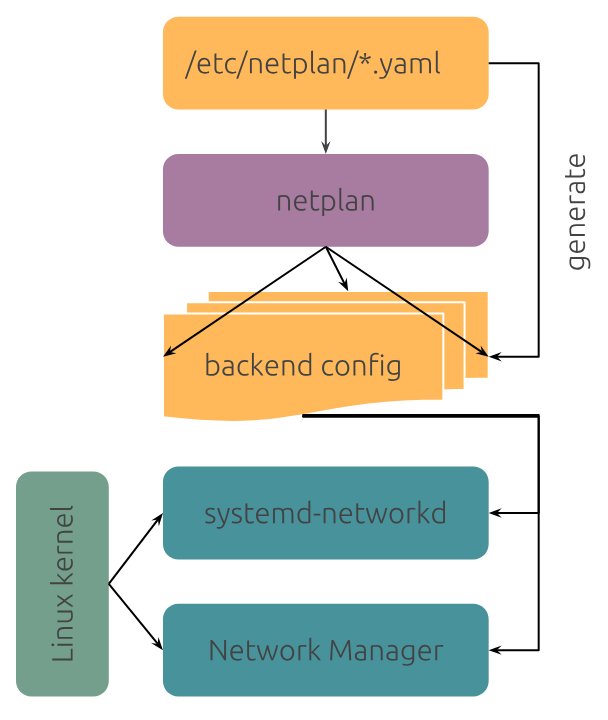
\includegraphics[width=0.4\linewidth]{Diagrams/os-netplans-hld.png}
    \caption{Netplan Design Overview}
    \parencite{Ubuntu2024NetplanDesign}
    \label{fig:netplan_design}
\end{figure}

\begin{figure}[H]
    \centering
    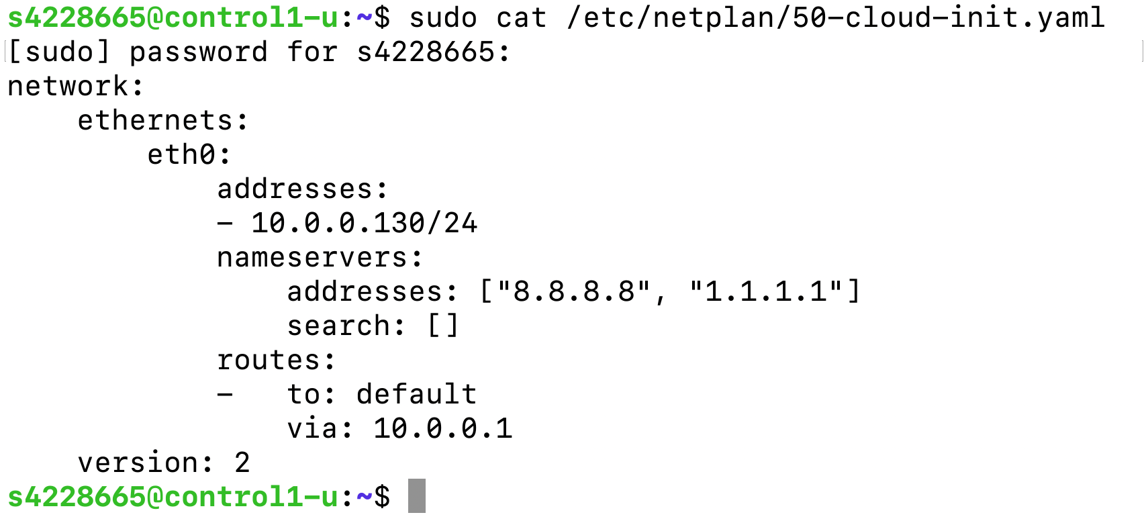
\includegraphics[width=0.75\linewidth]{Report_Images/os-netplan-screenshot.png}
    \caption{A netplan file}
    \label{fig:netplan-example}
\end{figure}

A rendered netplan file (figure \ref{fig:netplan_design}) showing a Pi's network config from the \verb|eth0| interface connected to network \verb|10.0.0.0/24| with IPv4 address \verb|10.0.0.130| using DNS servers \verb|8.8.8.8| and \verb|1.1.1.1| (owned and maintained by Google and Cloudfare), no search domain configured and default gateway (default route) at \verb|10.0.0.1|. This example was taken from the same Raspberry Pi (not the coursework-provided one) as shown in figure \ref{fig:UFW-example}.

\subsection{System Requirements and Design}
\label{subsec:system-requirements}

\subsubsection{Hardware Requirements}
As the firewall device is implemented using Ubuntu Server, base hardware requirements are incredibly low, sitting at:
\begin{itemize}
    \item 1.5 GB of RAM
    \item 5 GB of storage
\end{itemize}
While these are minimum specs, it would be better to have more resources than these; the Ubuntu docs mention having 3 GB (or more) of RAM and 25 GB (or more) for storage as recommended \parencite{Ubuntu2024SystemRequirements}. As for CPU specs, the official website does not even specify a CPU constraint/requirement. It instead shows supported 64-bit and 32-bit architectures which are:
\begin{itemize}
    \item amd64 (64-bit Intel/AMD)
    \item amd64 (64-bit Arm) - This is the type of CPU Raspberry Pi has
    \item armhf (32-bit Arm)
    \item ppc64el (64-bit Power)
    \item riscv64 (64-bit RISC-V)
    \item s390x (64-bit Mainframe)
\end{itemize}

\subsubsection{Hardware Overview}
The Raspberry Pi provided for this coursework is a Model 4B (with 4GB of RAM). This model has the following hardware specs:
\\Processing and Memory:
\begin{itemize}
    \item SoC: Broadcom BCM2711, Quad-core ARM Cortex-A72 (ARMv8) 64-bit @ 1.8 GHz
    \item RAM: 4 GB LPDDR4-3200 SDRAM
    \item GPU: VideoCore VI (not used)
\end{itemize}
\\Network Interfaces:
    \begin{itemize}
    \item Onboard Gigabit Ethernet
    \item WiFi: Dual-band 802.11ac WiFi (2.4 GHz and 5.0 GHz)
    \item Bluetooth: Bluetooth 5.0, BLE (not used)
\end{itemize}
\\Expansion and Connectivity:
\begin{itemize}
    \item USB Ports: 2× USB 3.0 ports, 2× USB 2.0 ports (The USB 3 ports are used for the additional NIC)
    \item GPIO: 40-pin header (not used)
    \item Display: 2× micro-HDMI ports (not used past OS install)
    \item Storage: microSD card slot
\end{itemize}

\subsubsection{Network Interface Card Overview}
As shown in figure \ref{basic-fw-breakdown} and the coursework brief, there should be 3 network interface cards (NICs), each configured to have a different class network represented. The Raspberry Pi firewall is able to accommodate this with the two onboard NICs and an additional WiFi NIC provided with the Pi.
\paragraph{Interface 1 - WAN/Class A Network}
\begin{itemize}
    \item Hardware: Onboard Gigabit Ethernet port
    \item Linux Device/Name: \verb|eth0|
    \item Connection: Physically cabled up with an RJ45 cat6e cable
    \item Summary: 
\end{itemize}

\paragraph{Interface 2 - LAN2/Class B Network}
\begin{itemize}
    \item Hardware: Additional WiFi Dongle NIC
    \item Linux Device/Name: ???
    \item Connection:
    \item Summary: 
\end{itemize}

\paragraph{Interface 3 - LAN2/Class C Network}
\begin{itemize}
    \item Hardware:
    \item Linux Device/Name: \verb|wlan0|
    \item Connection:
    \item Summary: 
\end{itemize}










\subsubsection{Iptables and Netfilter Requirements}
Iptables is a userspace utility that accesses the Netfilter module in the kernel, so it does not have its own system overhead. It is a command-line interface to configure the Linux kernel's Netfilter module/framework directly. The netfilter project is a community-driven, collaborative, free and open-source software (FOSS) project that provides packet filtering, NAT, packet logging, and other packet management for the Linux 2.4.X and later Kernels \parencite{Netfilter2024Official}.

Netfilter itself operates as a kernel module (not the userspace), which means packet filtering happens in the kernel space, so 'standard' use of the Pi would be unaffected by the packet inspection, similar to how an enterprise router would work with a control plane (userspace) and a forwarding plane (kernel space) \parencite{Cloudflare2024ControlPlane}. As such, the only requirement is the Ubuntu 24.04 (the latest long-term support (LTS)) operating system has Linux kernel 2.4 or later built in - this has been supported for years, and the Linux kernel in Ubuntu 24.04 is 6.8 \parencite{Ubuntu2024KernelLifecycle}.